%%%%%%%%%%%%%%%%%%%%%%%%%%%%%%%%%%%%%%%%%
% Beamer Presentation
% LaTeX Template
% Version 1.0 (10/11/12)
%
% This template has been downloaded from:
% http://www.LaTeXTemplates.com
%
% License:
% CC BY-NC-SA 3.0 (http://creativecommons.org/licenses/by-nc-sa/3.0/)
%
%%%%%%%%%%%%%%%%%%%%%%%%%%%%%%%%%%%%%%%%%

%----------------------------------------------------------------------------------------
%	PACKAGES AND THEMES
%----------------------------------------------------------------------------------------

\documentclass{beamer}

\mode<presentation> {

% The Beamer class comes with a number of default slide themes
% which change the colors and layouts of slides. Below this is a list
% of all the themes, uncomment each in turn to see what they look like.

%\usetheme{default}
%\usetheme{AnnArbor}
%\usetheme{Antibes}
%\usetheme{Bergen}
%\usetheme{Berkeley}
%\usetheme{Berlin}
%\usetheme{Boadilla}
%\usetheme{CambridgeUS} % preferred 2 red
%\usetheme{Copenhagen}
%\usetheme{Darmstadt}
%\usetheme{Dresden}
%\usetheme{Frankfurt}
%\usetheme{Goettingen}
%\usetheme{Hannover}
%\usetheme{Ilmenau}
%\usetheme{JuanLesPins}
%\usetheme{Luebeck}
%\usetheme{Madrid}
%\usetheme{Malmoe}
%\usetheme{Marburg}
%\usetheme{Montpellier}
%\usetheme{PaloAlto}
%\usetheme{Pittsburgh}
%\usetheme{Rochester}
\usetheme{Singapore}	%preferred 1
%\usetheme{Szeged}
%\usetheme{Warsaw}


% As well as themes, the Beamer class has a number of color themes
% for any slide theme. Uncomment each of these in turn to see how it
% changes the colors of your current slide theme.

%\usecolortheme{albatross}
%\usecolortheme{beaver}
%\usecolortheme{beetle}
%\usecolortheme{crane}
%\usecolortheme{dolphin}
%\usecolortheme{dove}
%\usecolortheme{fly}
%\usecolortheme{lily}
%\usecolortheme{orchid}
%\usecolortheme{rose}
%\usecolortheme{seagull}
%\usecolortheme{seahorse}
%\usecolortheme{whale}
%\usecolortheme{wolverine}

%\setbeamertemplate{footline} % To remove the footer line in all slides uncomment this line
%\setbeamertemplate{footline}[page number] % To replace the footer line in all slides with a simple slide count uncomment this line

%\setbeamertemplate{navigation symbols}{} % To remove the navigation symbols from the bottom of all slides uncomment this line
}

\usepackage{graphicx} % Allows including images
\usepackage{booktabs} % Allows the use of \toprule, \midrule and \bottomrule in tables
\usepackage{epstopdf} % Allows to view .eps files
\usepackage{amsmath}
\usepackage{amssymb}
\usepackage{color, flexisym}
\usepackage{epstopdf}
\usepackage{pdfpages}
\usepackage{epsfig}
\usepackage{breqn}

%----------------------------------------------------------------------------------------
%	TITLE PAGE
%----------------------------------------------------------------------------------------

\title[Dynamic TFA of C.Elegans]{Transcription Factor Activity of \textit{C. elegans}: \\From Probabilistic Markov model to\\ Gaussian process model} % The short title appears at the bottom of every slide, the full title is only on the title page

\author{Muhammad Arifur Rahman \\ Supervisor: Prof. Neil D. Lawrence} % Your name
\institute[SITraN] % Your institution as it will appear on the bottom of every slide, may be shorthand to save space
{
Department of Computer Science \\and\\ Sheffield Institute for Translational Neuroscience \\ The University of Sheffield \\ % Your institution for the title page
\medskip
\textit{M.Rahman@dcs.shef.ac.uk} % Your email address
}
\date{\today} % Date, can be changed to a custom date

\begin{document}

\begin{frame}
\titlepage % Print the title page as the first slide
\end{frame}

\begin{frame}
\frametitle{Overview} % Table of contents slide, comment this block out to remove it
\tableofcontents % Throughout your presentation, if you choose to use \section{} and \subsection{} commands, these will automatically be printed on this slide as an overview of your presentation
\end{frame}

%----------------------------------------------------------------------------------------
%	PRESENTATION SLIDES
%----------------------------------------------------------------------------------------

%------------------------------------------------
\section{Introduction} % Sections can be created in order to organize your presentation into discrete blocks, all sections and subsections are automatically printed in the table of contents as an overview of the talk

%------------------------------------------------
%------------------------------------------------
\subsection{Motivations} % A subsection can be created just before a set of slides with a common theme to further break down your presentation into chunks

%------------------------------------------------
%------------------------------------------------

\begin{frame}
\frametitle{Motivations}

\begin{figure}[t]
	\centering
		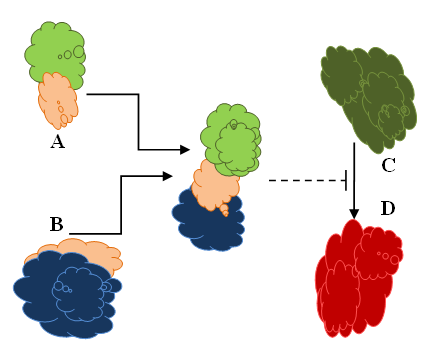
\includegraphics[scale=.35]{diagrams/ProtienProtien.png}
		\caption{A ‘cartoon’ model of protein protein interaction. Two different molecular species A and B bind to
		 form a complex molecular. The newly formed complex hinder the rate at which molecules of species 
		 C are transformed to species D.}
	\label{fig:Protein protein interaction}
\end{figure}


\end{frame}

%------------------------------------------------
\begin{frame}
\frametitle{Motivations}
\begin{figure}[t]
	\centering
		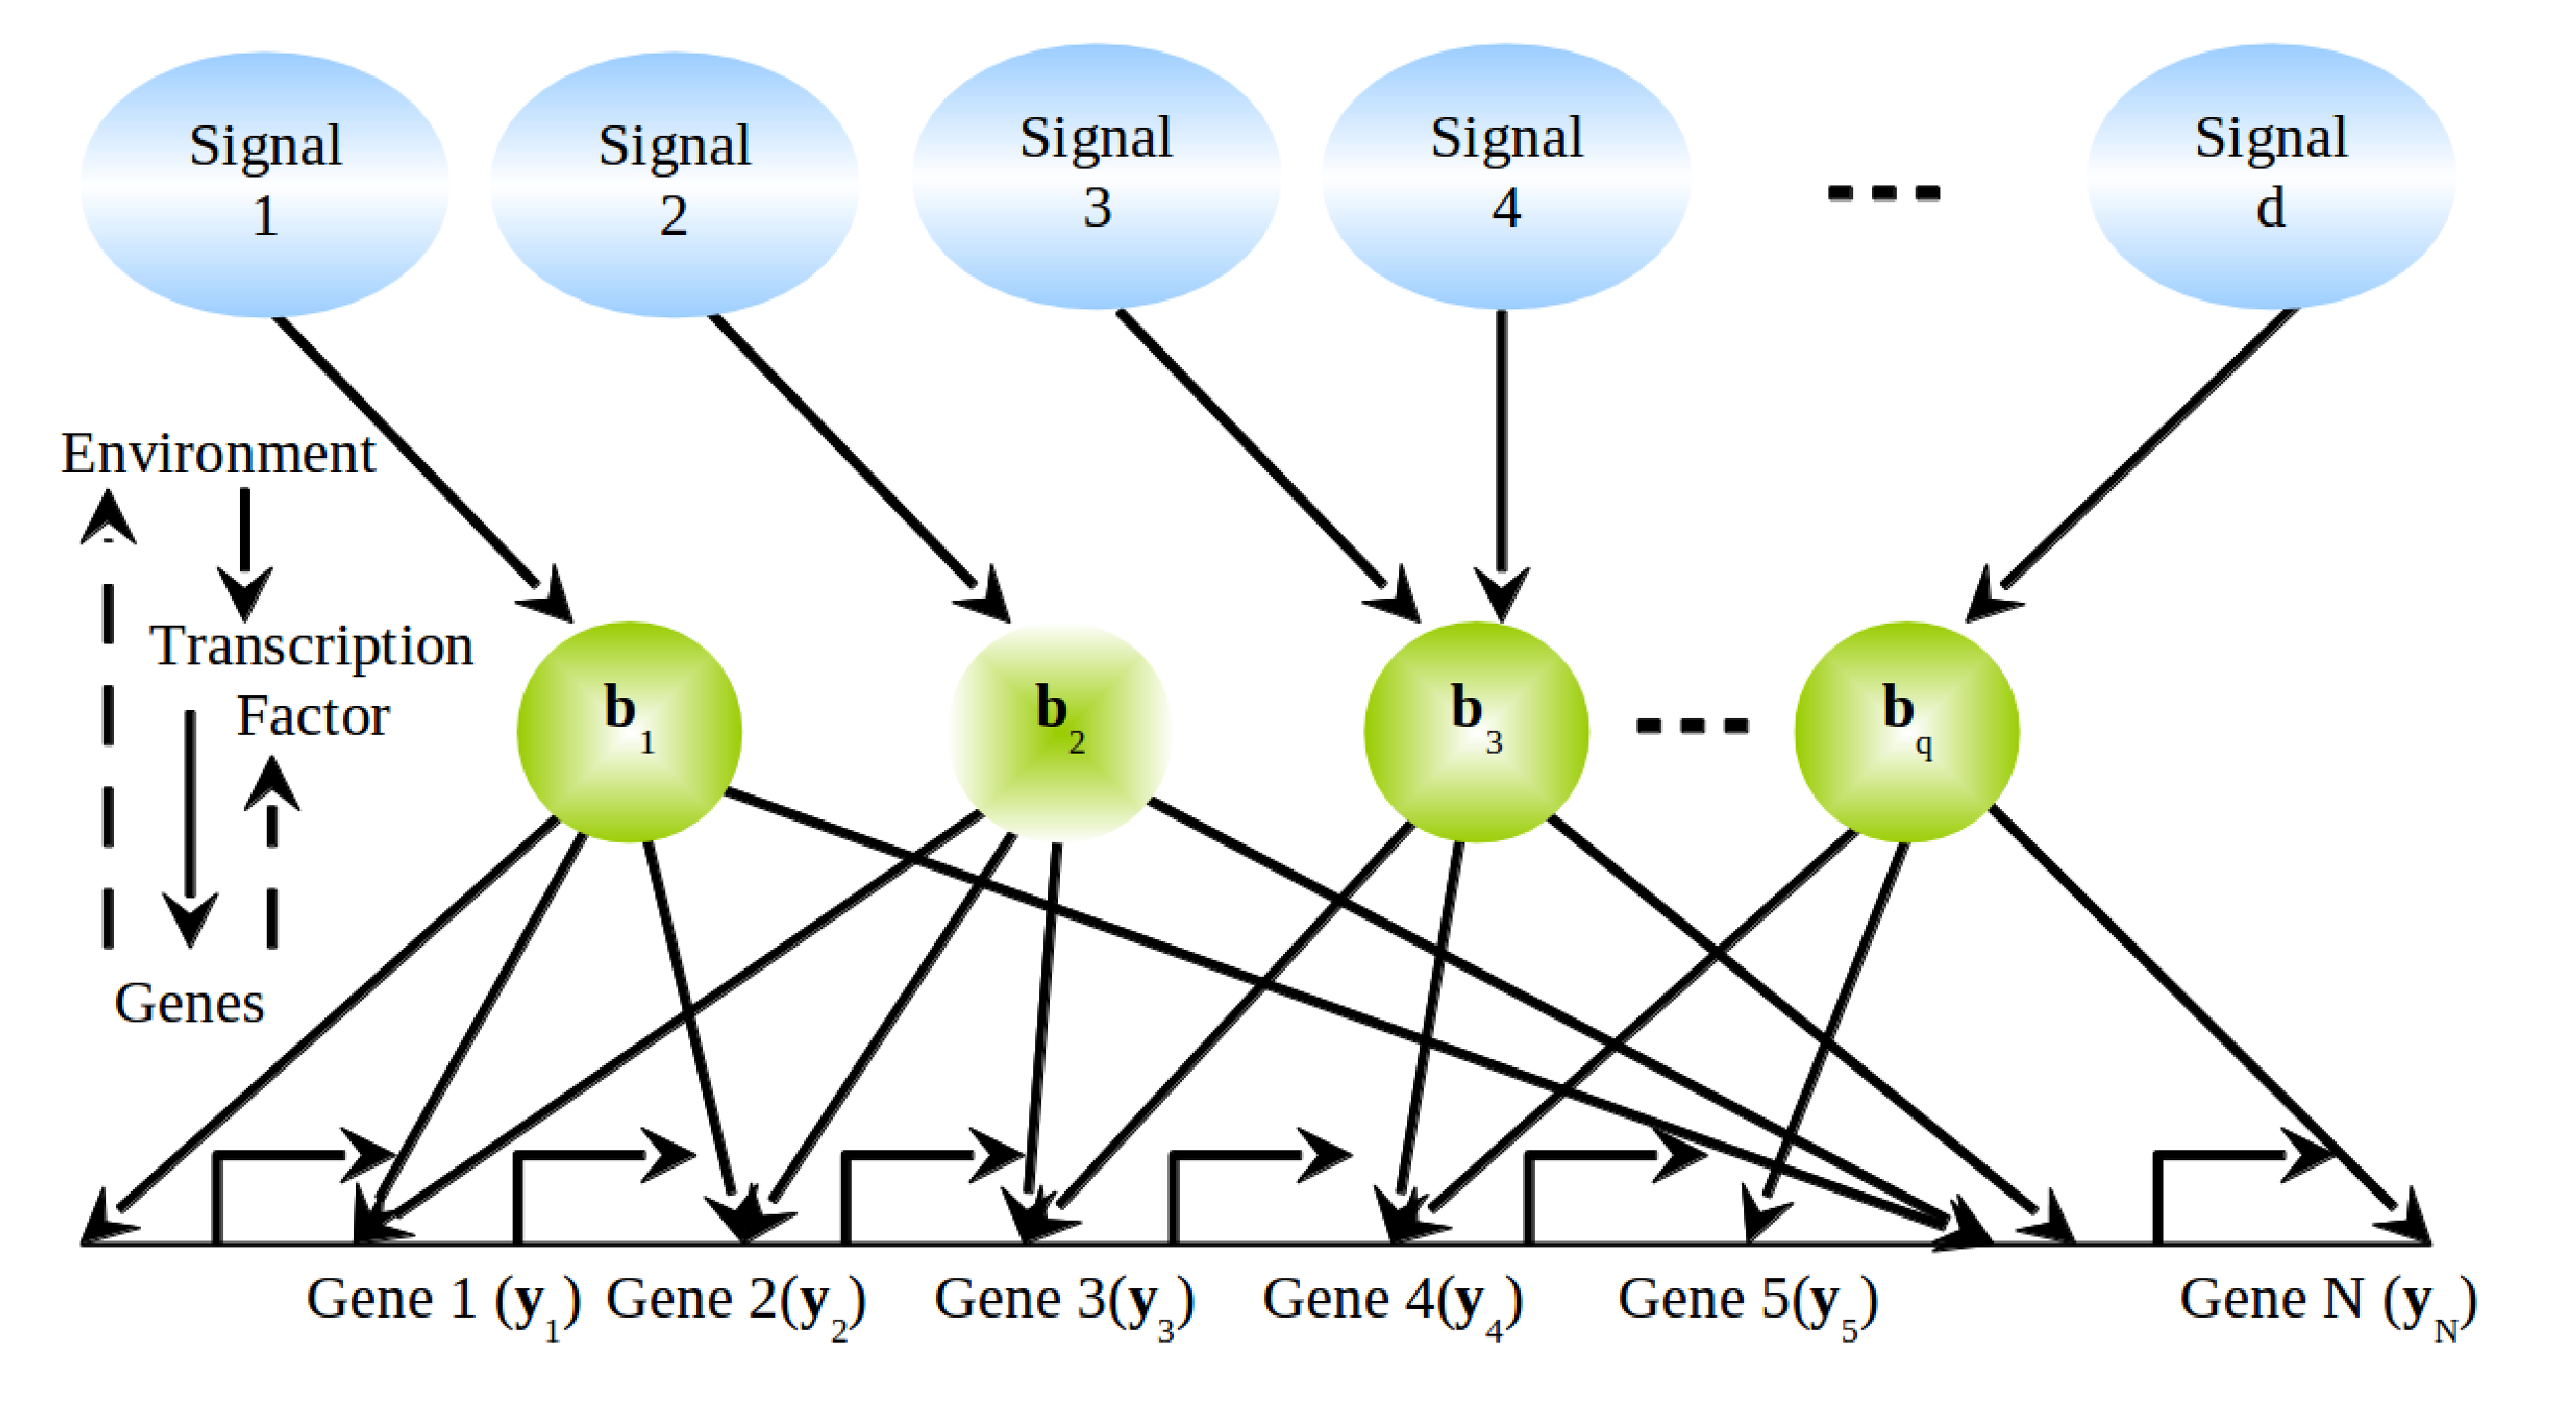
\includegraphics[width=0.75\textwidth,keepaspectratio]{diagrams/MappingEnvironmentalSignal.eps}
		\caption[The mapping between environmental signal, transcription factor inside 			the cell the genes that they regulate]{A 'cartoon' representation of mapping between environmental signal, transcription factor inside the cell the genes that they regulate.}
	\label{fig:MappingEnvironmentalSignal}
\end{figure}
\end{frame}
%------------------------------------------------


%------------------------------------------------

%------------------------------------------------
\begin{frame}
\frametitle{\textit{C. elegans} and Transcription Process}
\begin{columns}[c] % The "c" option specifies centered vertical alignment while the "t" option is used for top vertical alignment

\column{.45\textwidth} % Left column and width

\begin{itemize}
\item {Eukaryotic cells \color{green}$ \sim $ 1000} 
\item {Neurons \color{green} $ \sim $ 300} 
\item {Genes \color{red} $ \sim $ 15,139}
\item {TF \color{red} $ \sim $ 940}
\end{itemize}

%------------------------------------------------
\begin{figure}
\centering
	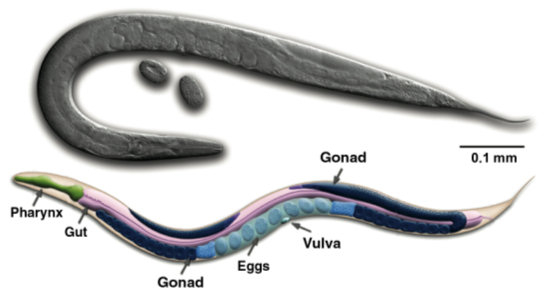
\includegraphics[scale=.2]{diagrams/celegans_image2.jpg}
	\caption{\textit{C. elegans}}
	\label{fig:cElegans}
\end{figure}

\column{.5\textwidth} % Right column and width
\begin{figure}[t]
\centering
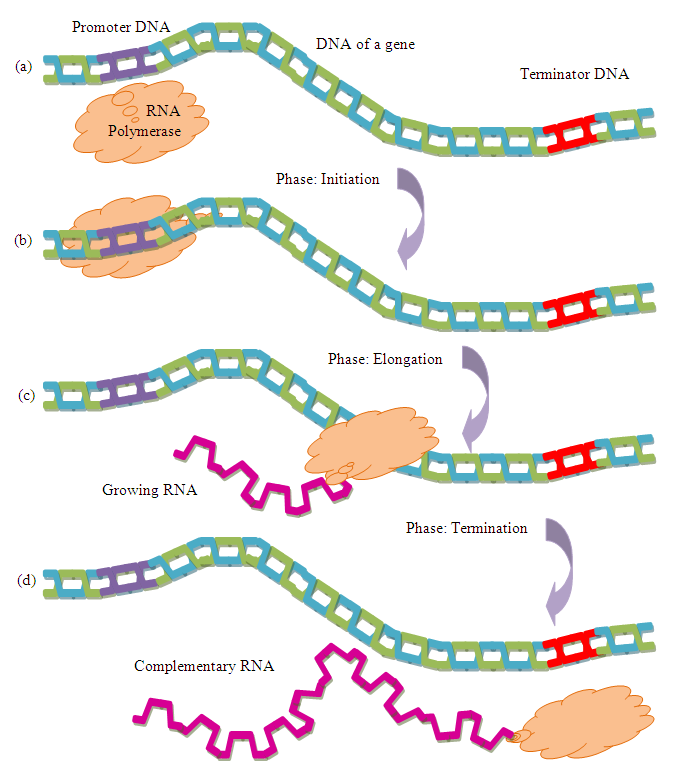
\includegraphics[scale=.22]{diagrams/transcriptionProcess.png}
%\caption{Transcription Process}
\label{fig:transcriptionProcess}
\end{figure}

\end{columns}
\end{frame}


%------------------------------------------------
\begin{frame}
\frametitle{Key Research Questions (Initial stage)}
\begin{itemize} 
\item Using existing mechanistic model can we step forward to find out the transcription factor activities of multicellular eukaryote (from a unicellular microorganism)? \\~\\

%\item Can we develop a robust data driven dynamic system for gene specific transcription factor activities using Gaussian process over a mechanistic model?

\end{itemize}
\end{frame}

%------------------------------------------------
\section{Probabilistic Model with Markov property}
\begin{frame}
\frametitle{Probabilistic Model with Markov property}
Our basic approach follows a dynamic model that extends the 
{\color{green} Linear Regression Model} of  \cite{p1}  and 
{\color{blue} Probabilistic Model} of  \cite{p2} to model the distribution of each transcription factor acting on each gene.\\~\\

Let, Gene expression- $ \bold{Y} \in \Re^{N \times d} $;  
Connectivity matrix- $ \bold{X} \in \Re^{N \times q} $ \\
TFAs can be obtained by regressing the gene expressions using the connectivity information, giving the following linear model- \\
\centering { $ \bold{y_{n}} = \bold{B_{n}} \bold{x_{n}} + \boldsymbol{\epsilon_{n}}$ } \\

Here $n = 1, . . . ,N$ indexes the gene, $ \bold{y_{n}} = \bold{Y}(n,:)^T $, $ \bold{x_{n}} = \bold{X}(n,:)^T $ and  $ \boldsymbol{\epsilon_{n}} $ is an error term. The ${d \times q}$ matrix $ \bold{B_{n}} $ models the gene specific TFAs. TFA for gene $n$ at any time $(t+1)$ is-

\centering {\color{red} $ \bold{b}_{n(t+1)} \sim \mathcal{N} (\gamma\bold{b}_{nt} + (1-\gamma)\boldsymbol{\mu},(1-\gamma^2)\boldsymbol{\Sigma})$} \\
for $ t= 1, ... , (d-1)$ and $ \bold{b}_{n1} \sim \mathcal{N} ( \boldsymbol{\mu},\boldsymbol{\Sigma})$

\end{frame}


%------------------------------------------------
%------------------------------------------------
\subsection{Data and Preprocessing}
%------------------------------------------------
%------------------------------------------------

\begin{frame}
\frametitle{Data Set: Gene Expression and Transcription Factors} 
\textbf{Gene Expression level:}
The point estimate of the expression level and the uncertainty of the expression level were extracted from the micro array data using the tool {\color{blue}puma} ~\cite{p6}.\\~\\  

\textbf{Transcription Factors:}
\textit{C. elegans} differential gene expression database {\color{blue}(EDGEdb)} \cite{{p7}} is the storage and retrieval of protein-DNA interactions. EDGEdb contains the sequence information of \textit{C. elegans}'s 934 transcription
factor and their DNA binding domains. 
\end{frame}


%------------------------------------------------
\begin{frame}
\frametitle{Data Set: Connectivity between Genes and TF}
Evidence code of Wormnet \footnote{http://www.functionalnet.org/wormnet/about.html} and ~\cite{p5} represent {\color{blue} different (21) types of relations} between genes.
We choose the following four relations to get the connectivity between genes and transcription factors-
\begin{itemize}
	  \item High-throughput yeast 2-hybrid assays among worm genes
	  \item Co-expression among worm genes
	  \item High-throughput yeast 2-hybrid assays among human genes
	  \item Literature curated human protein physical interactions 
\end{itemize} 

These relations leads to create a {\color{red} binary matrix} of {\color{blue} 0}'s and {\color{blue} 1}'s. 
\[
    x_{i,j}= 
\begin{cases}
    1,& \text{if } $\text {transcription factor $j$ can bind gene $i$ }$\\
    0,              & \text{otherwise}
\end{cases}
\] 
\end{frame}


%------------------------------------------------
%------------------------------------------------
\subsection{Result analysis}
\begin{frame}
\frametitle{Gene Specific TFA of {\color{red} hmg-4}{\footnote{High Mobility Group- 4 is required for locomotion and larval development}} (Sequence: T20B12.8)} %T20B12.8}
\begin{figure}
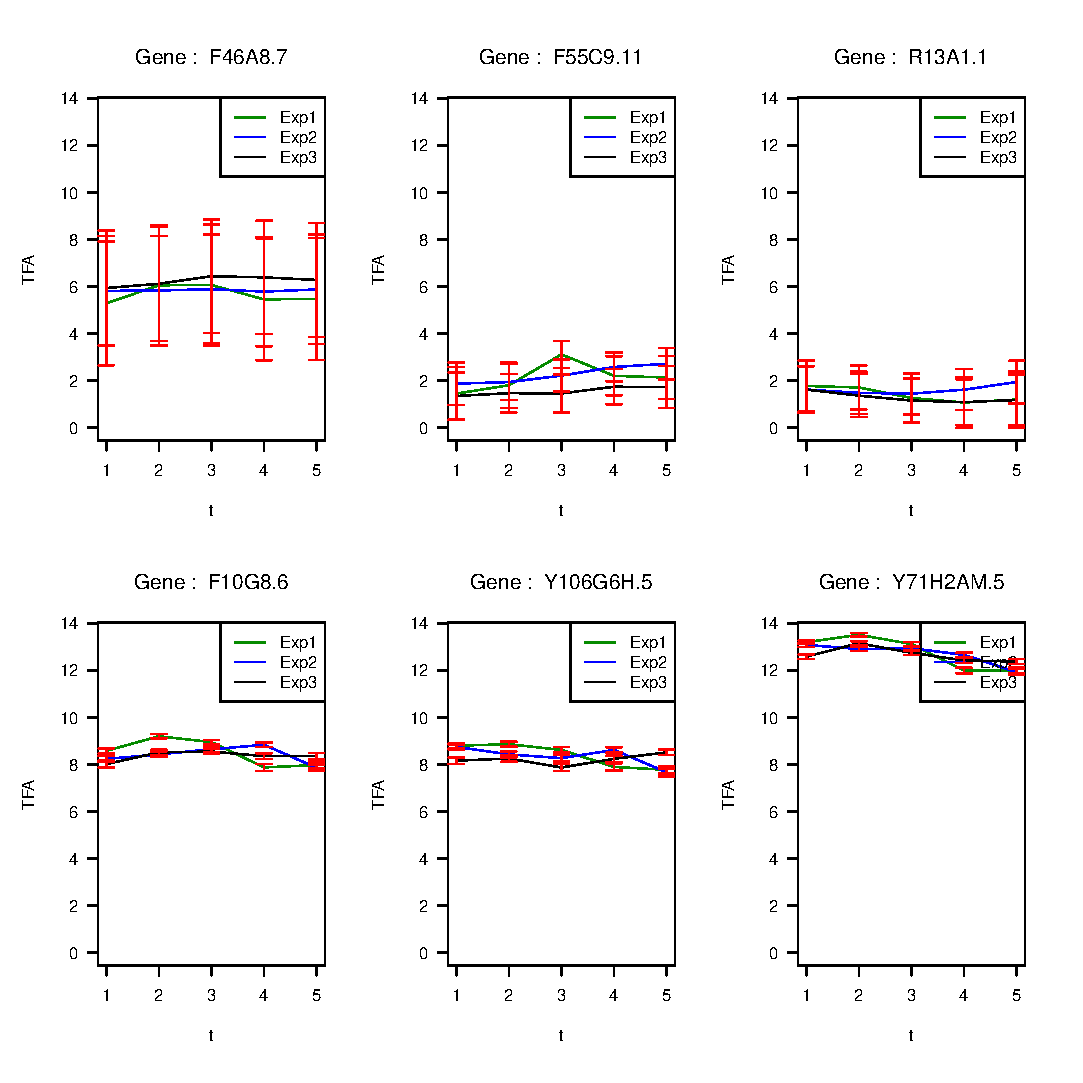
\includegraphics[width=0.65\linewidth]{diagrams/T20B12_8_3.eps}
%\caption{Figure caption}
\end{figure}
\end{frame}

%------------------------------------------------
\begin{frame}
\frametitle{Ranking Differentially expressed gene expressions and correlation between them}
\begin{figure}[t]
	\centering
		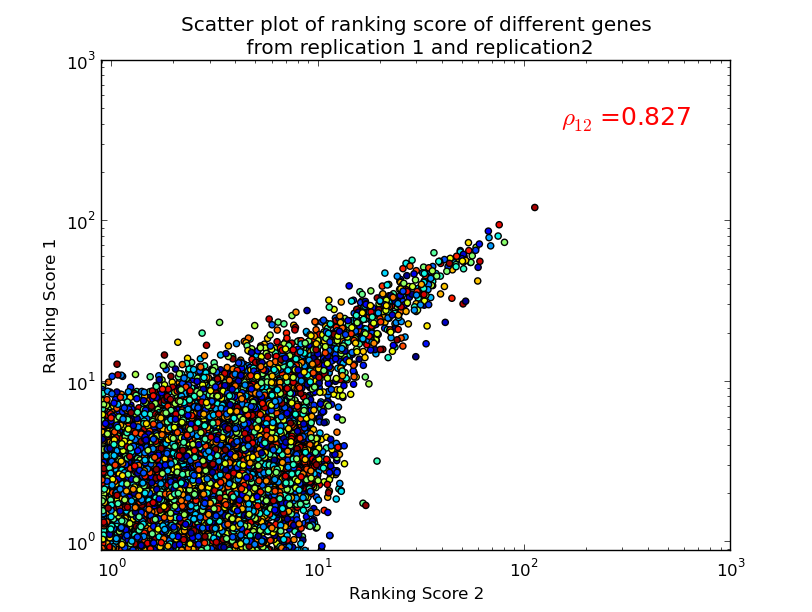
\includegraphics[scale=.3,keepaspectratio]{diagrams/RankingScore12.png}
		\caption[Pearson's correlation between different ranking scores]
		{Scatter plot of ranking score of different genes from replication 1 and replication 2 and Pearson's correlation}
	\label{fig:ranking_scores}
\end{figure}

\end{frame}

%------------------------------------------------
\begin{frame}
\frametitle{Examples of Genes regulated by multiple TF}
\begin{table}
\begin{tabular}{l l }
\toprule
\textbf{Gene Name/Sequence} & \textbf{Regulators activity} \\
\midrule

{\color{red} zip-8 (F23F12.9)} & {\color{blue} K10D2.3 }= $ 3.083311 \pm 0.239013 $, \\~\\ 


{\color{red} pitp-1 (M01F1.7)} & {\color{blue} F38A5.13 }= $ 0.714906468 \pm 0.2790247 $, \\ 
		       & {\color{blue} T24C4.7} = $ 0.006439146 \pm 0.1516683 $ \\~\\


{\color{red} ssp-33 (R08A2.3)} & {\color{blue} T19B10.11} = $ 0.5793706446 \pm 1.1397625 $ \\
		  & {\color{blue} W02D7.6} = $ 0.5793706446 \pm 1.1397625 $ \\
 		  & {\color{blue} D1014.8} = $ 0.0004742555 \pm  0.0438619 $\\~\\

{\color{red} C38D4.1} & {\color{blue} ZC513.6} = $ 0.9681545 \pm  0.4944999 $ \\
		  & {\color{blue} T04C10.4 } = $ -0.4815358 \pm  1.0099097 $ \\
 		  & {\color{blue} M01E11.5 } = $ -0.5252536 \pm  0.4952643 $ \\
		  & {\color{blue} Y11D7A.12 } = $ -6.3354545 \pm 1.4231987 $ \\
\bottomrule
\end{tabular}
\caption{Genes regulated by multiple TF}
\end{table}
\end{frame}


%------------------------------------------------

\begin{frame}
\frametitle{Active TF in different clusters of Microarray Data}
\begin{columns}[c] % The "c" option specifies centered vertical alignment while the "t" option is used for top vertical alignment

\column{.32\textwidth} % Right column and width
\begin{figure}[!htb]
\centering
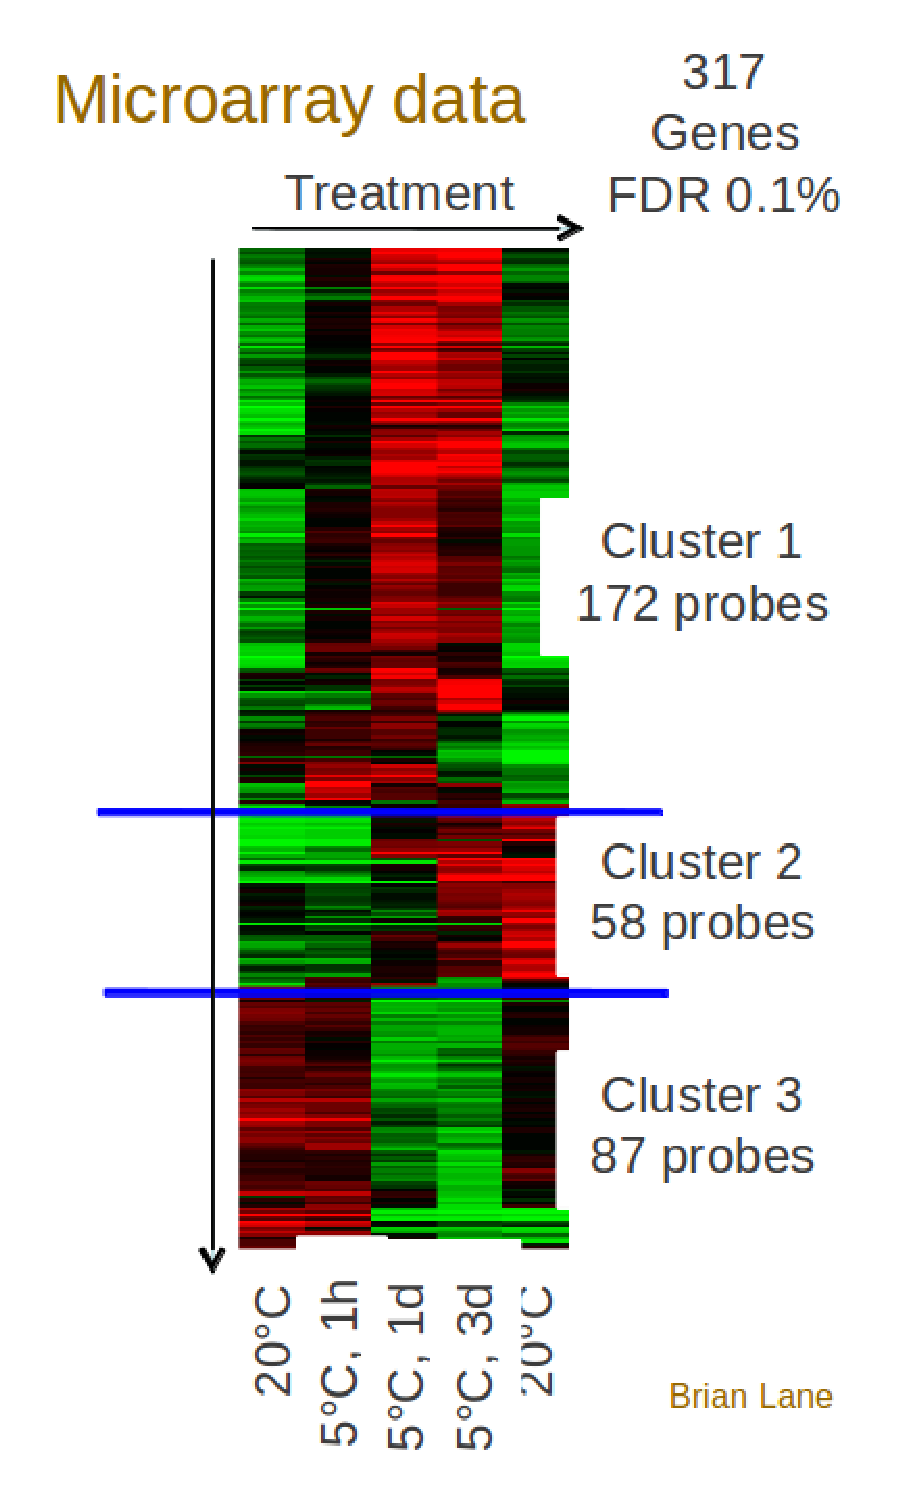
\includegraphics[scale=.27]{diagrams/mcd2.eps}
\label{fig:Microarray Data}
\end{figure}

\column{.6\textwidth} %Left column and width

\begin{table}
\begin{tabular}{l l }
\toprule
\textbf{{\color{red}Cluster} \color{blue}Name} & \textbf{Active TF} \\
\midrule

{\color{red}1} - {\color{blue}Chill upregulated} & 6 \\ 
{\color{red}2} - {\color{blue}Chill late upregulated} & 245 \\ 
{\color{red}3} - {\color{blue}Chill downregulated genes} & 128 \\
{\color{red}4} - {\color{blue} Others} & 203 \\

\bottomrule
\end{tabular}
\caption{Number of Transcription Factor active in different Clusters}
\end{table}

\end{columns}
\end{frame}

%------------------------------------------------


\begin{frame}
\frametitle{Key Research Questions (Secondary stage)}
\begin{itemize} 
\item  Using existing mechanistic model can we step forward to find out the transcription factor activities of multicellular eukaryote (from a unicellular microorganism)? \\
\hfill {\color{green}\textbf{Yes}; Our $R$ based $chipDyno$ tool is ready!} \\~\\
\item {Can we develop a robust data driven dynamic system for gene specific transcription factor activities using Gaussian process over a mechanistic model?} 

\end{itemize}
\end{frame}

%------------------------------------------------
\section{GP Model}
%\subsection{Defination}
%------------------------------------------------
%------------------------------------------------
\begin{frame}
\frametitle{Gaussian Process (Definition)}
A Gaussian process is a collection of random variables, any finite number of which have a joint Gaussian distribution\footnote{Rasmussen and Williams}. It is a continuous stochastic process and defines probability distributions for functions.

If $f(\textbf{x})$ is a real process, a Gaussian process is completely defined by its mean function and covariance function given by-
\begin{equation} \label{eq:GP}
f\left(\textbf{x} \right)\sim \mathcal{GP} \left(m \left(\textbf{x}\right), k \left(\textbf{x},\textbf{x\textprime}\right) \right).
\end{equation}

The mean function $m(\textbf{x})$  and the covariance function $k(\textbf{x},\textbf{x\textprime})$ are defined as-
\begin{equation} \label{eq:2.3}
m(\textbf{x})= \mathbb{E}[f(\textbf{x})],
\end{equation}
\begin{equation} \label{eq:2.4}
k(\textbf{x},\textbf{x\textprime})= 
\mathbb{E}[(f(\textbf{x})-m(\textbf{x}))(f(\textbf{x}\textprime)-m(\textbf{x}\textprime))],
\end{equation}
where $\mathbb{E}$ represents the expected value.

\end{frame}

%------------------------------------------------
%------------------------------------------------
\subsection{Toward the GP model of TFA}
\begin{frame}
\frametitle{Toward the GP model of TFA}
In the earlier probabilistic approach gene specific TFAs was-
\begin{equation} \label{eq:tfa_SanG_updateCh4}
  {\color{red}\bold{b}_{n(t+1)} \sim \mathcal{N} (\gamma \bold{b}_{nt} + (1-\gamma)\boldsymbol{\mu},(1-\gamma^2)\bold{\Sigma})}
\end{equation}
For a {\color{blue}discrete time variable $k$} and a {\color{blue}one-dimensional process} with the property with $\mu$ and $s$ are scalar-
\begin{equation}
u_{k+1} \sim \mathcal{N}\left(\gamma u_k + \left(1 - \gamma\right) \mu, (1 - \gamma^2)s \right),
\end{equation}

Assume that {\color{blue}$u_k$'s are actually values $u_{t_k}$} from a continuous process $u(t)$ and $t_k = kDt$.
A good candidate for this kind of model is the mean-reverting $Ornstein-Uhlenbeck$ model-
\begin{equation}
du = -\lambda \left(u - \mu\right) dt + q^{1/2} dB,
\end{equation}
where $\lambda$ is mean reversion rate, $B$ is standard Brownian motion and $q$ is volatility. This equation can now be solved on the time instants $t_k$ and the result is a recursion
\begin{equation}
{\color{blue}u(t_k) = a u(t_{k-1}) + b \mu + w_{k-1}}; where, w_{k-1} \sim \mathcal{N}(0,c)
\end{equation}
 
\end{frame}

%------------------------------------------------
\begin{frame}
\frametitle{Toward the GP model of TFA(Cont..)}
We can now match the coefficients:
\begin{equation} \label{eq:a}
a = \exp(-\lambda Dt) = \gamma
\end{equation}
\begin{equation} \label{eq:b}
b = 1 - \exp(-\lambda Dt) = 1 - \gamma
\end{equation}
\begin{equation} \label{eq:c}
c = [q / (2 \lambda)] [1 - \exp(-2 \lambda Dt)]= (1 - \gamma^2) s 
\end{equation}

We can now recall that the (stationary) covariance function of the Ornstein-Uhlenbeck process we get-
\begin{equation}
k_u(t,t')= s \gamma^{\left|t-t'\right|}
\end{equation}
The original vector valued $\textbf{b}$, is separable, then the covariance function is obtained by formally replacing $s$ with 
$\boldsymbol{\Sigma}$ everywhere- 
\begin{equation}
\textbf{K}_b(t,t') = \boldsymbol{\Sigma} \boldsymbol{\gamma}^{\left|t-t'\right|}
\end{equation}

Thus is equivalent to considering the vector process- 
\begin{equation}
\textbf{db} = -\lambda (\textbf{b} - \boldsymbol{\mu}) \textbf{dt} + Q^{1/2} \textbf{dB}.
\end{equation}

\end{frame}

%------------------------------------------------
\subsection{GP model for TFA}
\begin{frame}
\frametitle{GP model for TFA}

Gene expression is $\mathbf{Y} \in \Re^{n\times T}$ and the unobserved corresponding TFA is $\mathbf{F}\in\Re^{q\times T}$.
Basic assumptions-
\begin{itemize}
\item TFA are in time series, they are likely to be temporally smooth. 
\item TF are potentially correlated with one another.
\end{itemize} 

\textbf{Correlation Between Transcription Factors}:  
The correlation between different TF is covariance matrix, $\boldsymbol{\Sigma}$ with $q\times q$ dimensionality. 

\textbf{Temporal Smoothness}: 
The TFs' activities is temporally smooth, and drawn from an underlying GP with covariance $\mathbf{K}_t$. 

\textbf{Intrinsic Coregionalization Model}: 
We assume that the joint process across all $q$ TFA and across all time points is well represented by an intrinsic model of coregionalization where the covariance is given by the 
Kronecker product of these terms.
\begin{equation} \label{eq:K}
  \mathbf{K}_f = \mathbf{K}_t \otimes \boldsymbol{\Sigma}
\end{equation}

\end{frame}

%------------------------------------------------
\begin{frame}
\frametitle{GP model for TFA(cont..)}

Assume that the $j$th gene's expression at the $i$th time point is given by-
\begin{equation} \label{eq:yij}
  \mathbf{y}_{i, j} = \mathbf{S}\mathbf{f}_{:, i} + \boldsymbol{\epsilon}_i
\end{equation}  
where, Gaussian noise- $\epsilon_i \sim \mathcal{N}(\mathbf{0}, \sigma^2 \mathbf{I})$ and $\mathbf{S}$ connectivity matrix.

From standard properties of multivariate Gaussian distributions-
\begin{equation} \label{eq:mGPd}
\mathbf{y} \sim \mathcal{N}(\mathbf{0}, \mathbf{K})
\end{equation}
\begin{equation} \label{eq:K}
\mathbf{K} = \mathbf{K}_t \otimes \mathbf{S} \boldsymbol{\Sigma} \mathbf{S}^\top + \sigma^2 \mathbf{I}.
\end{equation}
The likelihood of a multivariate Gaussian is:
\begin{equation} \label{eq:Likelihood}
L = -\frac{1}{2} \log |\mathbf{K}| - \frac{1}{2} \mathbf{y}^\top \mathbf{K}^{-1} \mathbf{y} =({\color{red}L_q}+{\color{blue}L_u}+Const)
\end{equation}
\begin{equation} \label{eq:Lq}
{\color{red}L_q} = -\frac{1}{2} \log |\mathbf{K}_t\otimes
	  \boldsymbol{\Lambda}\mathbf{V}^\top\boldsymbol{\Sigma}\mathbf{V}\boldsymbol{\Lambda}+\sigma^2\mathbf{I}| 
	- \frac{1}{2} \hat{\mathbf{y}}_q^\top \left[\mathbf{K}_t\otimes 
	  \boldsymbol{\Lambda}\mathbf{V}^\top\boldsymbol{\Sigma}\mathbf{V}\boldsymbol{\Lambda}+\sigma^2\mathbf{I}\right]^{-1} \hat{\mathbf{y}}_q
\end{equation}
\begin{equation} \label{eq:Lu}
{\color{blue}L_u} = -\frac{T(n-q)}{2} \log \sigma^2  -\frac{1}{2\sigma^2} \hat{\mathbf{y}}_u^\top \hat{\mathbf{y}}_u
\end{equation}

\end{frame}

%------------------------------------------------
\begin{frame}
\frametitle{GP model for TFA: Making Prediction}

Using Kronecker product, Rotation, SVD and considering noise we can rewrite the Equation \ref{eq:mGPd} as:
\begin{equation} \label{eq:predicYq}
  \mathbf{y_q}  \sim \mathcal{N} \left( \mathbf{0}, 
    \mathbf{K}_{t,t} \otimes \boldsymbol{\Lambda} \mathbf{V}^T\boldsymbol{\Sigma} \mathbf{V} \boldsymbol{\Lambda} +
    \sigma^2\mathbf{I}\right)
\end{equation}
To make predictions about the test data we need the conditional distribution- $p(\textbf{f}_\star|\textbf{y})$. This conditional distribution is also Gaussian-
\begin{equation} \label{eq:predicYq}
  \mathbf{f}_\star  \sim \mathcal{N} \left( \boldsymbol{\mu}_F, \boldsymbol{C}_F \right)
\end{equation}

The mean of the posterior distribution of Equation \ref{eq:predicYq} is:
\begin{equation} \label{eq:prediction_MuF}
  \boldsymbol{\mu}_F = 
    \mathbf{K}_{t_\star,t} \otimes \boldsymbol{\Sigma} \mathbf{V} \boldsymbol{\Lambda}
    \left[ \mathbf{K}_{t,t} \otimes \boldsymbol{\Lambda} \mathbf{V}^T\boldsymbol{\Sigma} \mathbf{V} \boldsymbol{\Lambda} + \sigma^2 \mathbf{I} \right]^{-1}\mathbf{y}_q
\end{equation}

Covariance of the posterior distribution of Equation \ref{eq:predicYq} %\ref{eq:predictionTFA} 
given by:

\begin{dmath}
%\begin{equation} \label{eq:prediction_CF}
  \boldsymbol{C}_F = 
    \mathbf{K}_{t_\star,t_\star} \otimes \boldsymbol{\Sigma} -
    \mathbf{K}_{t_\star,t} \otimes \boldsymbol{\Sigma}\mathbf{V} \boldsymbol{\Lambda}
    \left[ \mathbf{K}_{t,t} \otimes \boldsymbol{\Lambda} \mathbf{V}^T\boldsymbol{\Sigma} \mathbf{V} \boldsymbol{\Lambda} + \sigma^2 \mathbf{I} \right]^{-1} 
    \left[ \mathbf{K}_{t_\star,t} \otimes \boldsymbol{\Lambda} \mathbf{V}^T\boldsymbol{\Sigma}\right]
%\end{equation}
\end{dmath}


\end{frame}
%------------------------------------------------
\subsection{Result analysis}
\begin{frame}
\frametitle{Covariance Matrix and TFA}
\begin{columns}[c] 
\column{.5\textwidth} % Left column and width
\begin{figure}[t]
	\centering
		%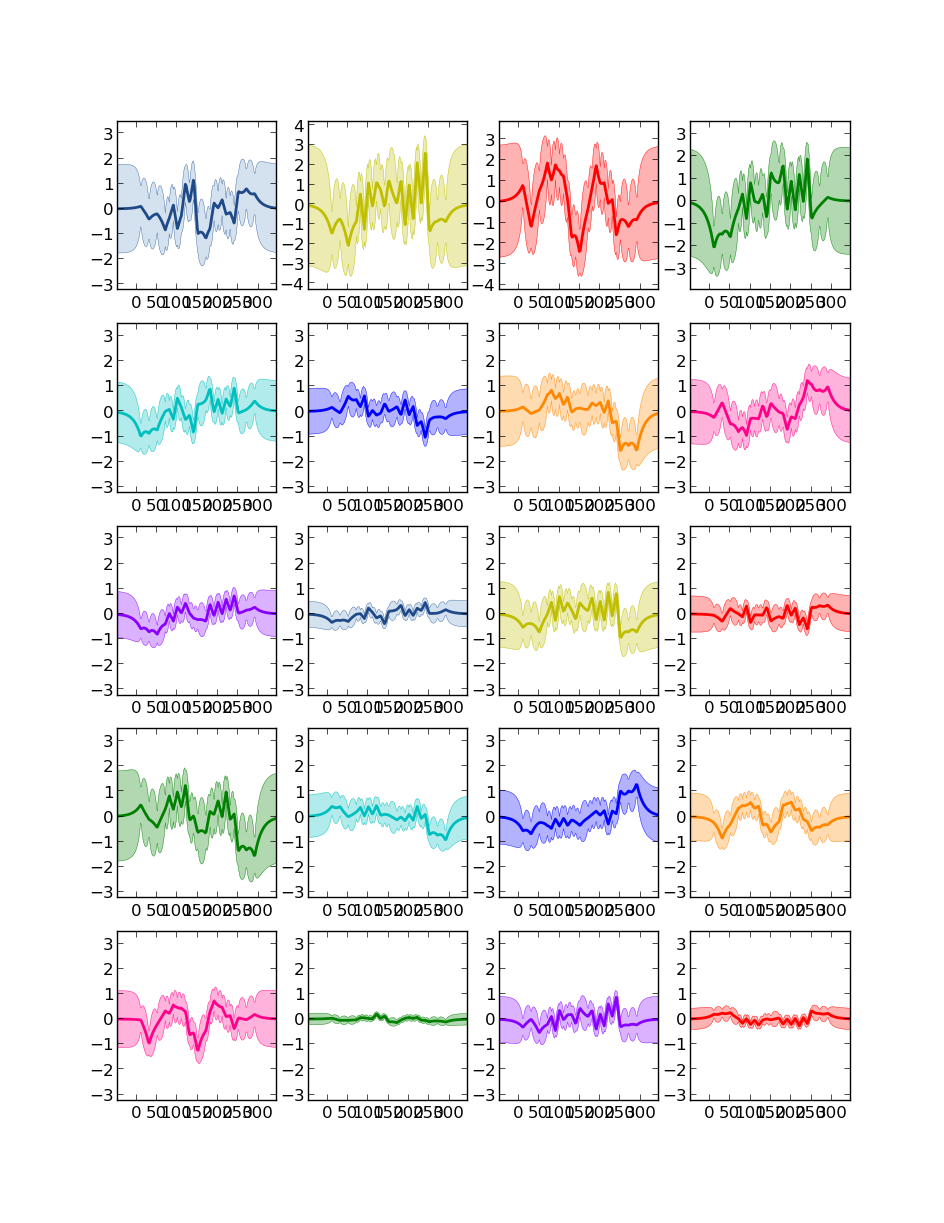
\includegraphics[width=17cm,keepaspectratio]{diagrams/OU20TF.png}
		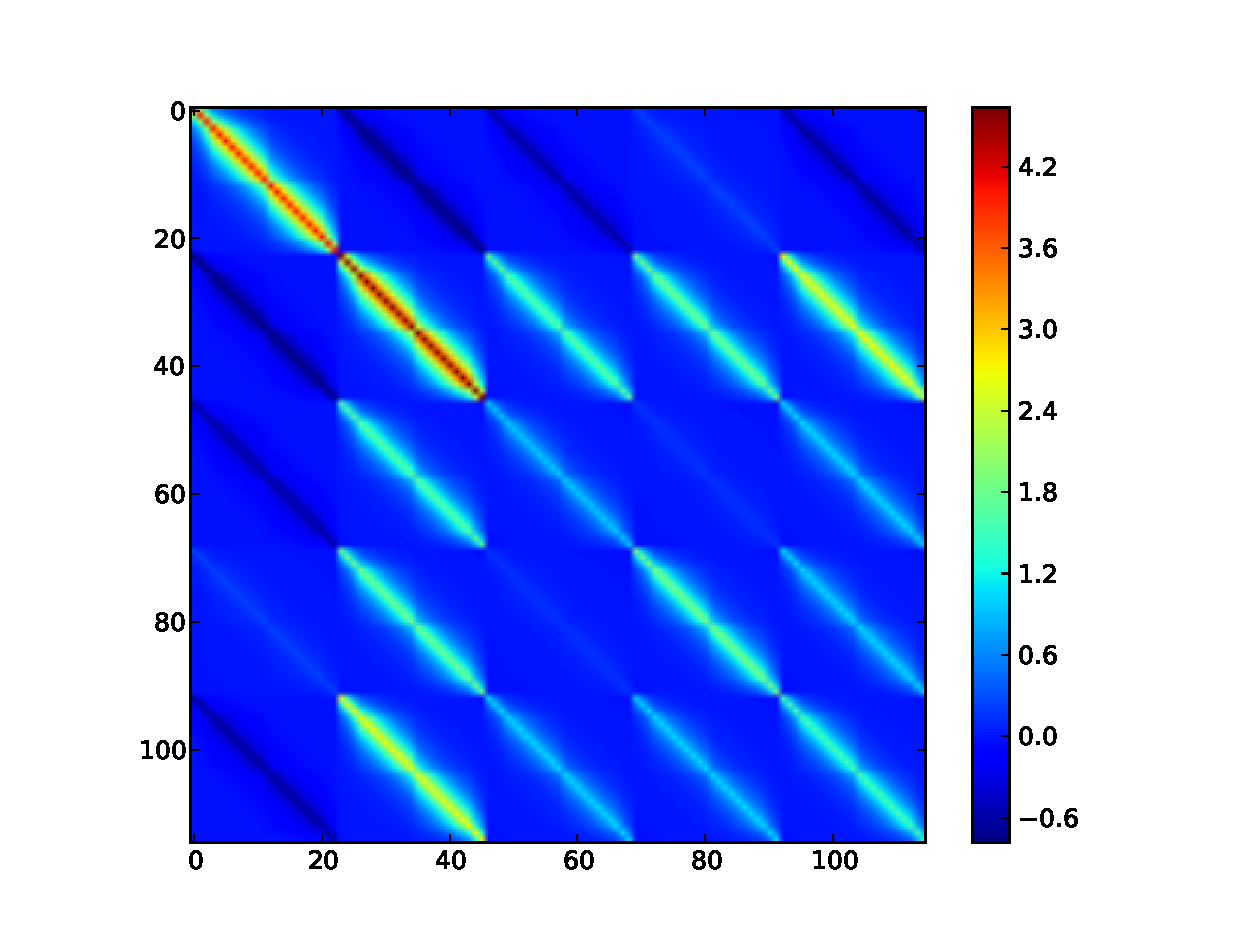
\includegraphics[width=.8\textwidth,keepaspectratio]{diagrams/kern_6TF.eps}
	\caption[Kernel of Intrinsic Coregionalization model $\textbf{K}_f$ considering 5 
		 Transcription factors where covariance matrix $\boldsymbol{\Sigma}$
		 was constructed using Ornstein-Uhlenbeck kernel and White kernel in additive form]
		{Kernel of Intrinsic Coregionalization model $\textbf{K}_f$ considering 5 
		 Transcription factors where covariance matrix $\boldsymbol{\Sigma}$ 
		 of $\left( Equation \ref{eq:K} \right)$ was constructed 
		 using Ornstein-Uhlenbeck kernel and White kernel in additive form}
	\label{fig:kern_6TF}
\end{figure}
\column{.5\textwidth} % Right column and width
\begin{figure}[]
	\centering
		%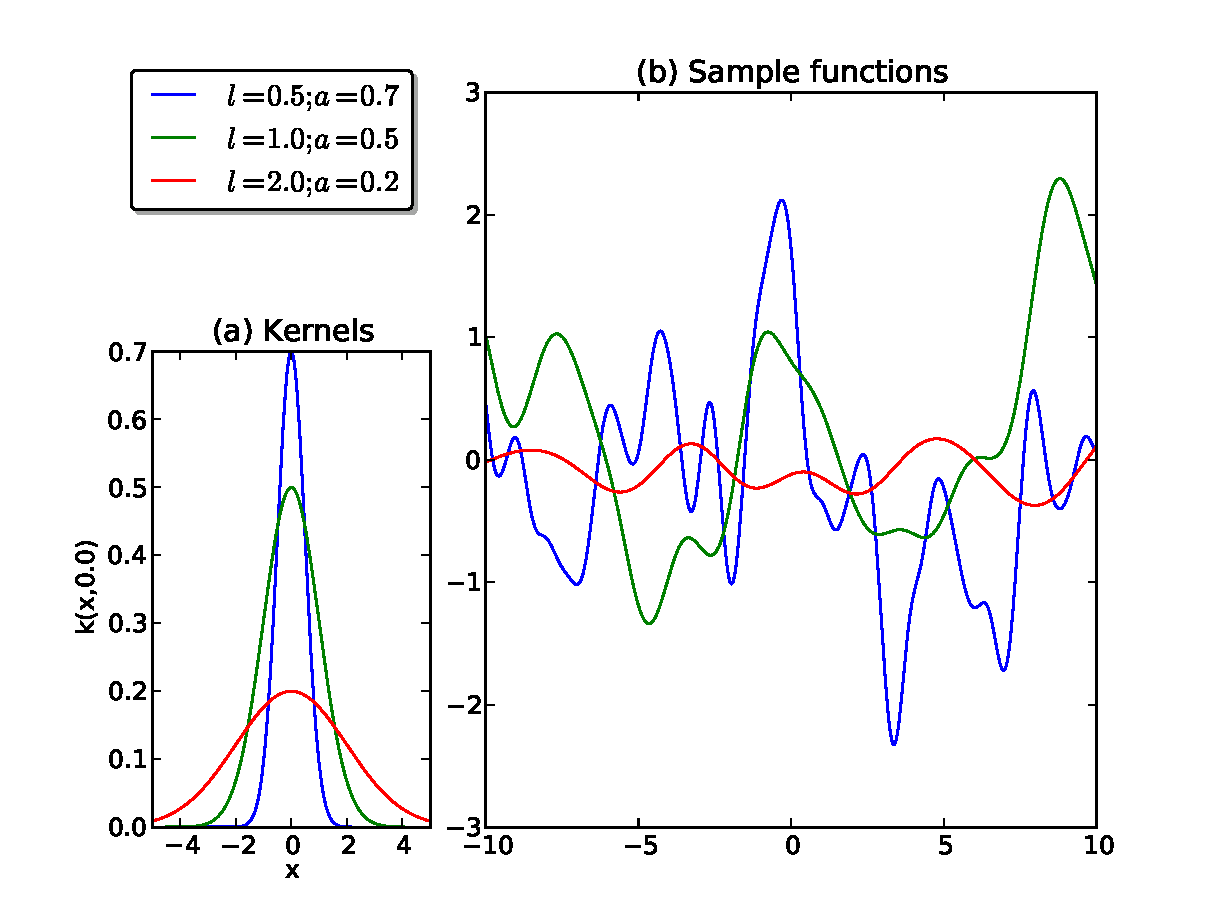
\includegraphics[width=10cm,keepaspectratio]{diagrams/SE_cov.pdf}
		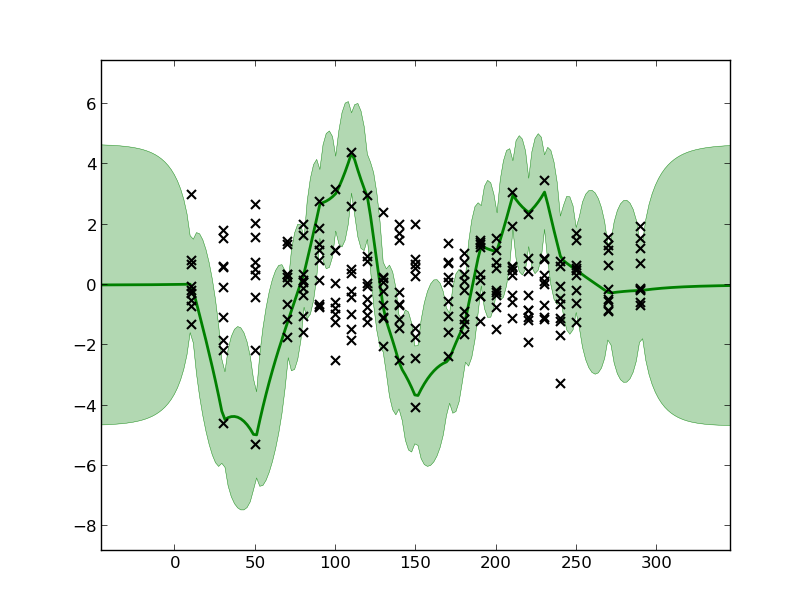
\includegraphics[width=0.9\textwidth,keepaspectratio]{diagrams/ACE2_OU_Wh_9TF.png}
	\caption[Transcription factor activity of ACE2]
		{Transcription factor activity of ACE2 shaded area represents 95\% confidence interval}
	\label{fig:TFA_of_of_ACE2}
\end{figure}

\end{columns}

\end{frame}

%------------------------------------------------

\begin{frame}
\frametitle{Transcription factor activity of different TF}
\begin{figure}[]
	\centering
		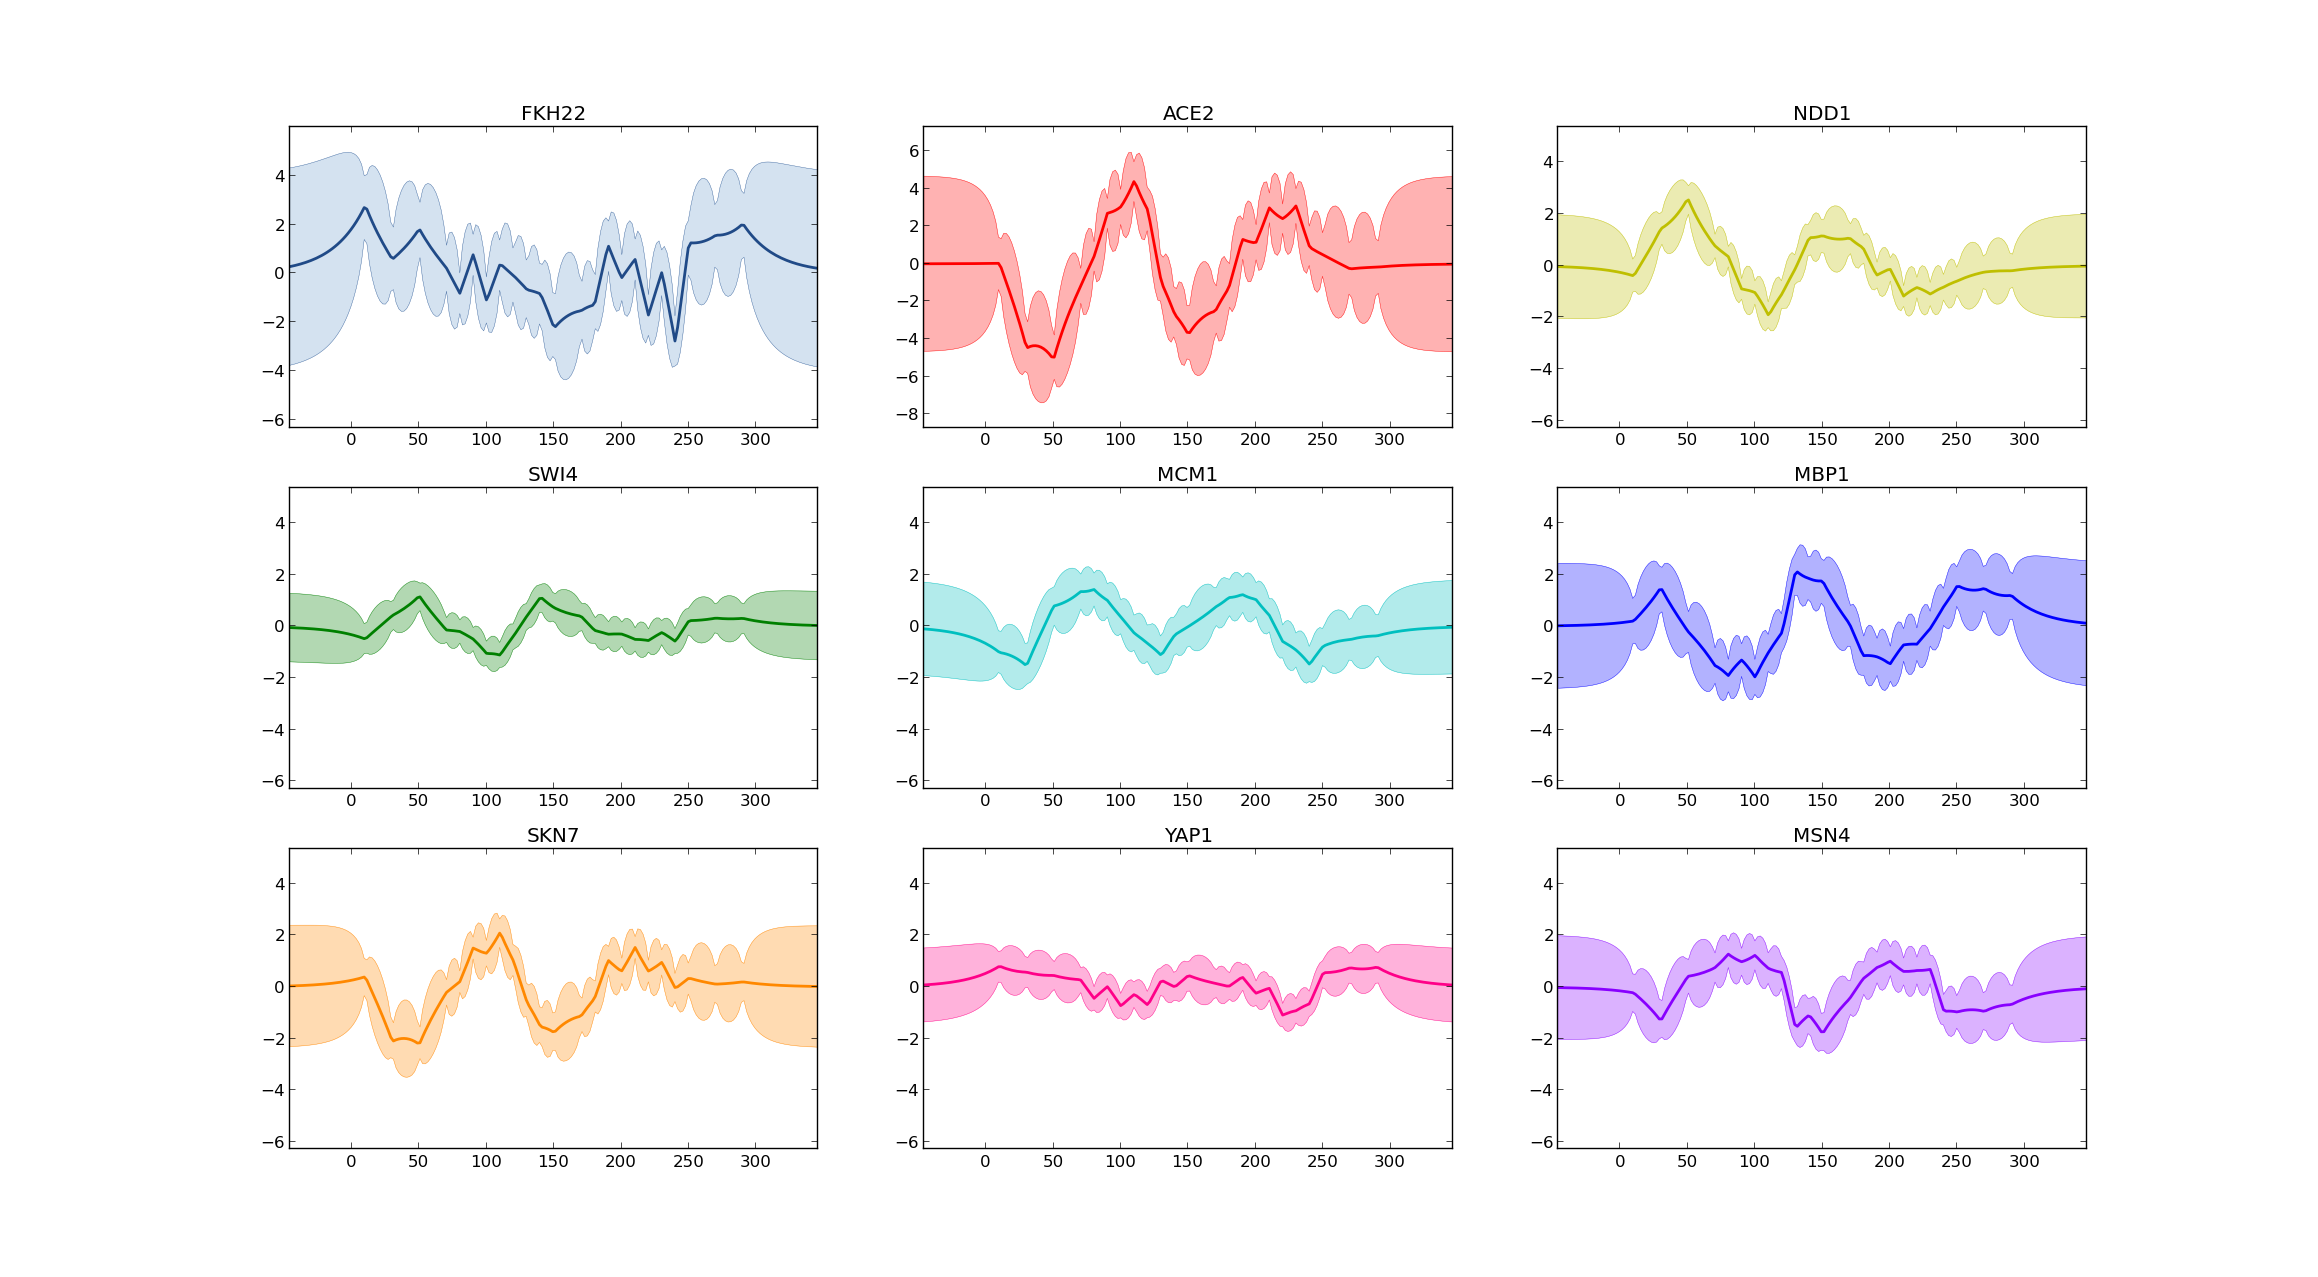
\includegraphics[width=\textwidth,keepaspectratio]{diagrams/OUWh9TF_Title.png}
	\caption[Transcription factor activity of different TF using Ornstein-Uhlenbeck kernel and White kernel]
		{Transcription factor activity of different TF using Ornstein-Uhlenbeck kernel and 
		White kernel in additive form}
	\label{fig:TFA_of_20TF}
\end{figure}

\end{frame}
%------------------------------------------------
\section{Conclusion and Future Work}
\subsection{Conclusion}
\begin{frame}
\frametitle{Conclusion}
\begin{itemize}
\item Our \emph{R} based tool \emph{chipDyno} integrate the connectivity information between genes and transcription factors, and microarray data and infer the TFA.
\item {\color{blue}Earlier the model was developed for a unicellular microorganism (yeast) but we were successful to determine the gene specific TFA for \textit{C. elegans}, a multicellular eukaryote.} 
\item We were also successful to filter out the quiet genes from the
differentially expressed genes for \textit{C. elegans}.
\item {\color{blue} Our GP model will overcome the restriction of parametric model and temporal sampling of equally spaced time intervals.}
\item ~38\% of the protein-coding genes orthologs of human genes; The biological insight acquire from \textit{C. elegans} may be directly applicable to more complex organism like human..
\end{itemize}
\end{frame}

%------------------------------------------------
\subsection{Future Work}
\begin{frame}
\frametitle{Future Work}
\begin{itemize}
\item Transgenic mice can express human SOD1 mutation and replicates different histopathological and clinical features of Motor Neurone Disease (MND). But we didn't found any evidence which analyse MND considering the genetic background on 
different phenotype. We will use our GP model to infer the TFA on gene expression data obtained from different murine models and try to find out some insights.
\item It is assumed that gene involved in the same biological 
process will be expressed with a similarity sharing underlying time series. Again it is very common to have multiple biological replicates of the gene expression. Just taking average of the replicates surely lead toward discarding insight. Using this GP based hierarchical clustering analysis we will find some robust clusters for the gene expression data of \textit{C. elegans}. 
\end{itemize}
\end{frame}

%------------------------------------------------
%------------------------------------------------
\section{References}
%------------------------------------------------
%------------------------------------------------
\begin{frame}[fragile] % Need to use the fragile option when verbatim is used in the slide
\frametitle{Acknowledgements}

\begin{itemize}
\item {\bf Prof. Andrew Cossins}, Institute of Integrative Biology, University of Liverpool for the data set and valuable suggestions. \\
\item {\bf Dr. Simo S\"arkk\"a}, Academy Research Fellow, Department of Biomedical Engineering and Computational Science, Aalto University. \\
\item {\bf puma} : The Bioconductor package. \\
\item {\bf GPy} : The Gaussian process framework. \\
\item {\bf Ministry of Science and Information Technology, Bangladesh} for funding the scholarship.

\end{itemize}


\end{frame}

%------------------------------------------------

\begin{frame}
\frametitle{References}
\footnotesize{
\begin{thebibliography}{70} % Beamer does not support BibTeX so references must be inserted manually as below

\bibitem[Liao, 2003]{p1} Liao, J.C. Liao JC, Boscolo R, Yang YL, Tran LM, Sabatti C, Roychowdhury VP. (2003)
\newblock Network component analysis: reconstruction of regulatory signals in biological systems.
\newblock \emph{Proc Natl Acad Sci U S A.} 2003 Dec 23;100(26):15522-7. Epub 2003 Dec 12.

\bibitem[Liu,X. et al. 2005]{p3} Liu,X. et al. (2005) 
\newblock A tractable probabilistic model for affymetrix probe-level analysis across multiple chips. 
\newblock \emph {Bioinformatics}, 21, 3637–3644.

\bibitem[Nachman,I. et al. 2004]{p4}Nachman,I. et al. (2004) \newblock Inferring quantitative models of regulatory networks from expression data. 
\newblock \emph{Bioinformatics}, 20, i248–i256.

\bibitem[Sanguinetti, 2006]{p2} Sanguinetti G, Rattray M., and Lawrence N.D. (2006)
\newblock A probabilistic dynamical model for quantitative inference of the regulatory mechanism of transcription
\newblock \emph{Bioinformatics, Oxford University Press,} Vol. 22 no. 14, pages 1753–1759

\bibitem[Lee, 2013]{p5} Insuk Lee, Ben Lehner, Catriona Crombie, Wendy Wang, Andrew G. Fraser and Edward M. Marcotte (2013)
\newblock Probabilistic functional gene network of Caenorhabditis elegans
\newblock \emph{"\url{http://www.functionalnet.org/wormnet/about.html}",} Online; accessed 03-November-2014

\bibitem[Barrasa, 2007]{p7} MI Barrasa, P Vaglio, F Cavasino, L Jacotot, AJ Walhout (2007)
\newblock EDGEdb: a transcription factor-DNA interaction database for the analysis of C. elegans differential gene expression.
\newblock \emph{BMC Genomics. 2007}, Jan 18;8:21.

\bibitem[Pearson,R. et al. 2009]{p6} R. Pearson and X. Liu and G. Sanguinetti and M. Milo and N.D. Lawrence and M. Rattray (2009) 
\newblock puma: a Bioconductor package for Propagating Uncertainty in Microarray Analysis. 
\newblock \emph {BMC Bioinformatics}, 10:211.

\end{thebibliography}
}
\end{frame}

%------------------------------------------------

\begin{frame}
%\Huge{\centerline{Thank You}}
\begin{figure}

\includegraphics[width=0.4\linewidth]{diagrams/question.png}
%\caption{Figure caption}
\end{figure}
\end{frame}


%------------------------------------------------
%------------------------------------------------
%------------------------------------------------
%------------------------------------------------

\begin{frame}
\frametitle{Motivations(Cont..)}
\begin{itemize}

\item In molecular biology and genetics, a transcription factor is a protein that binds to specific DNA sequence.
\item Transcription factors {\color{blue} control the flow} (or transcription) of genetic information from {\color{blue} DNA to mRNA}. 
\item To develop models of {\color{blue} cellular processes} quantitative estimation of the regulatory relationship between transcription factors and genes is a {\color{blue}basic requirement}. 
\item It is difficult for a number of reasons: transcription factors’ expression levels are often {\color{red} low and noisy}, and many transcription factors are {\color{red}post- transcriptionally regulated}. 
\item So, from the expression levels of their target genes it is functional to infer the activity of the transcription factors.

\end{itemize}
\end{frame}

%------------------------------------------------
\begin{frame}
\frametitle{\textit{Caenorhabditis elegans}}
\begin{columns}[c] % The "c" option specifies centered vertical alignment while the "t" option is used for top vertical alignment

\column{.45\textwidth} % Left column and width
\textbf{Some basic features-}
\begin{itemize}
\item Sydney Brenner (1927 - ) established C. Elegans as a model organism to study genetics and cell development.
\item Adults are ~1mm long.
\item They can be grown on agar plates with lawn of bacteria.
\item They have a short generation time- 3 days from egg-laying to adulthood. 
\end{itemize}

\column{.5\textwidth} % Right column and width
\begin{itemize}
\item {Number of eukaryotic cells \color{green}$ \sim $ 1000} 
\item {Number of neurons \color{green} $ \sim $ 300} 
\item {Number of genes \color{red} $ \sim $ 15,139} \footnote{http://www.functionalnet.org/wormnet/about.html}
\item {Number of Transcription factors \color{red} $ \sim $ 940} \footnote{ http://edgedb.umassmed.edu/TFFilesListingAction.do}
\end{itemize}

\begin{figure}[!htb]
\centering
	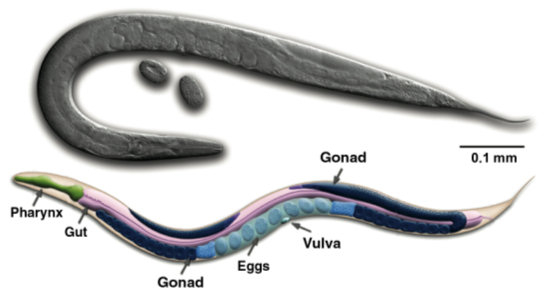
\includegraphics[scale=.2]{diagrams/celegans_image2.jpg}
	\caption{\textit{C. Elegans}}
	\label{fig:cElegans}
\end{figure}

\end{columns}
\end{frame}

%------------------------------------------------

\begin{frame}
\frametitle{Transcription}
\begin{columns}[c] % The "c" option specifies centered vertical alignment while the "t" option is used for top vertical alignment

\column{.45\textwidth} % Left column and width
\textbf{Some basic features-}
\begin{enumerate}
\item The information in DNA is not directly converted into proteins, but must first be copied into RNA
\item Transcription produces genetic messages in the form of mRNA.
\item During transcription, a DNA sequence is read by an RNA polymerase. 
\item Transcription produces a complementary, anti-parallel RNA strand
\end{enumerate}

\column{.5\textwidth} % Right column and width

\begin{figure}[!htb]
\centering
	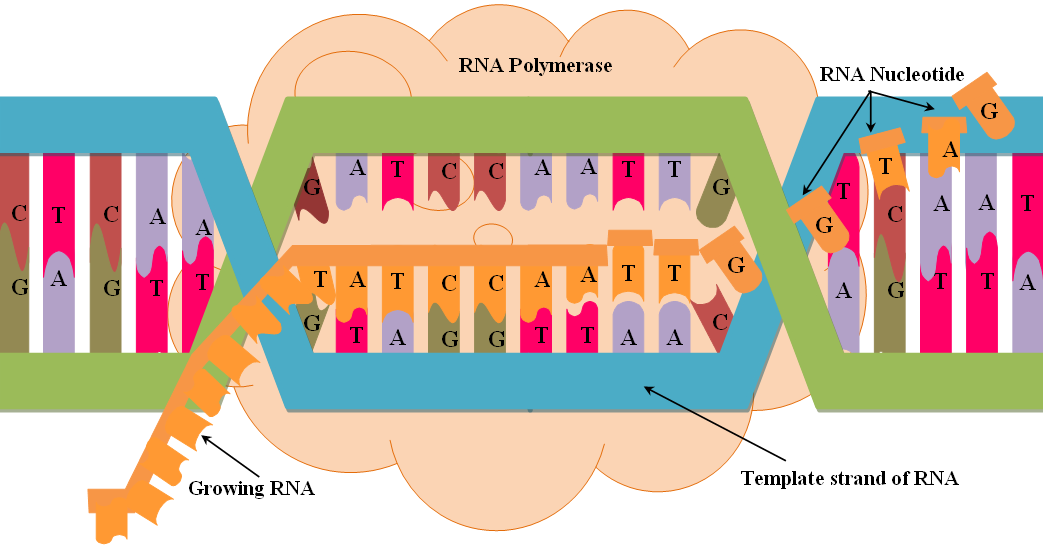
\includegraphics[scale=.16]{diagrams/Transcription.png}
	\caption{Transcription}
	\label{fig:transcription}
\end{figure}

\end{columns}
\end{frame}

%------------------------------------------------

\begin{frame}
\frametitle{Transcription Process}
\begin{columns}[c] % The "c" option specifies centered vertical alignment while the "t" option is used for top vertical alignment

\column{.45\textwidth} % Left column and width
%\textbf{Three main steps of transcription process-}
%\begin{itemize}
{\bf Initiation} : Transcription process starts at the promoter region of a double-stranded DNA. \\
{\bf Elongation} : A sequence specific DNA binding factors called {\color{red}transcription factors} then unwind the DNA strand\\
{\bf Termination} : Unwinding DNA's double helical form RNA polymerase reaches the terminator sequence. Here, RNA polymerase releases the mRNA polymer.
%\end{itemize}

\column{.5\textwidth} % Right column and width

\begin{figure}[t]
\centering
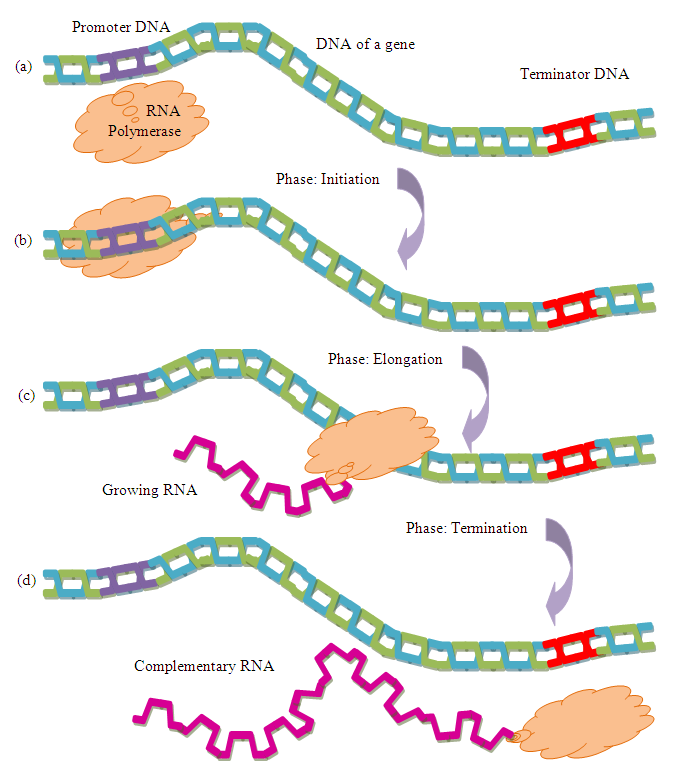
\includegraphics[scale=.24]{diagrams/transcriptionProcess.png}
%\caption{Transcription Process}
\label{fig:transcriptionProcess}
\end{figure}

\end{columns}
\end{frame}


%------------------------------------------------
%------------------------------------------------
\begin{frame}
\frametitle{Probabilistic Model(cont..)}

Two plausible assumptions for TFA-
\begin{itemize}
\item Firstly,  Gene specific TFA $ \bold{b}_{nt} $ at time $ t $ depends solely on the gene specific TFA at time $ (t-1) $. 
\item Secondly, it was assumed that the prior distribution to be a stationary in time. \\~\\
\end {itemize}

Two limiting case-
\begin{itemize}
\item The first limiting case, when experimental data set consists of replication of condition i.e. all the $ \bold{b}_{nt} $ assumed to be identical, so that- \\
\centering { $ \bold{b}_{n1} \sim \mathcal{N} ( \boldsymbol{\mu},\boldsymbol{\Sigma})$ and $ \bold{b}_{n(t+1)} \sim \mathcal{N} ( \bold{b}_{nt},\bold{0})$}
%\raggedleft
\raggedright
\item Second limiting case was when all the $ \bold{ b_{nt}} $ were assumed to be independent and identically distributed- \\ \centering {$ \bold{b}_{nt} \sim \mathcal{N} ( \boldsymbol{\mu},\boldsymbol{\Sigma})$}

\end{itemize}
\end{frame}

%------------------------------------------------

\begin{frame}
\frametitle{Probabilistic Model(cont..)}

\begin{itemize}
\item  \cite{p2}  expected a realistic model of time series data to be somewhere in between this two extremes- \\
\centering $ \bold{b}_{n(t+1)} \sim \mathcal{N} (\boldsymbol{\gamma}\bold{b}_{nt} + (1-\gamma)\boldsymbol{\mu},(1-\gamma^2)\boldsymbol{\Sigma})$ \\
for $ t= 1, ... , (d-1)$ and $ \bold{b}_{n1} \sim \mathcal{N} ( \boldsymbol{\mu},\boldsymbol{\Sigma})$
\raggedright
\\ Where $ \gamma $ is a parameter measuring the degree of temporal continuity of the TFAs \\~\\

\item Likelihood function-\\
\centering 
$p(\bold{Y|B,X})= \displaystyle \prod_{n \mathop = 1}^{N} p(\bold{y_n|B_n,x_n})$

\raggedright
\item TFAs can be estimated a posteriori using Bayes' Theorem- \\~\\
\centering 
$ p(\bold{b_n|Y})= \frac {p(\bold{Y|b_n})p(\bold{b_n})}{p(\bold{Y})} $

\end {itemize}
\end{frame}

%----------------------------------------------------------------------------------------
%------------------------------------------------

\begin{frame}

\frametitle{How the clusters were made?}

{\color{red} Cluster 1} - {\color{blue} Chill upregulated:}  
cell morphogenesis, cell growth, regulation of cell size, electron transport, regulation of cell growth, generation of precursor metabolites and energy, anatomical structure,  morphogenesis, cellular metabolic process, proteolysis\\~\\

{\color{red}Cluster 2} - {\color{blue} Chill late upregulated:}
chromosome organization and biogenesis, DNA packaging, chromatin architecture, chromatin modification, negative regulation of developmental process, chromatin remodeling regulation of developmental process, DNA metabolic process, larval development (sensu Nematoda), organelle organization and biogenesis, post-embryonic development\\~\\

{\color{red} Cluster 3} - {\color{blue} Chill downregulated genes:} 
amino acid and derivative metabolic process, carboxylic acid metabolic process, organic acid metabolic process, fatty acid metabolic process, amino acid metabolic process, monocarboxylic acid metabolic process

\end{frame}

%------------------------------------------------

\begin{frame}
\frametitle{Covariance function and Kernels Representation}

\begin{columns}[c] 
\column{.5\textwidth} % Left column and width
\textbf{Exponentiated Quadratic covariance function}
\begin{equation} \label{eq:EQ_cov}
K_{EQ}(r)= a^2 \exp \left(-\frac{r^2}{2l^2}\right)
\end{equation}
\begin{figure}[t]
	\centering
		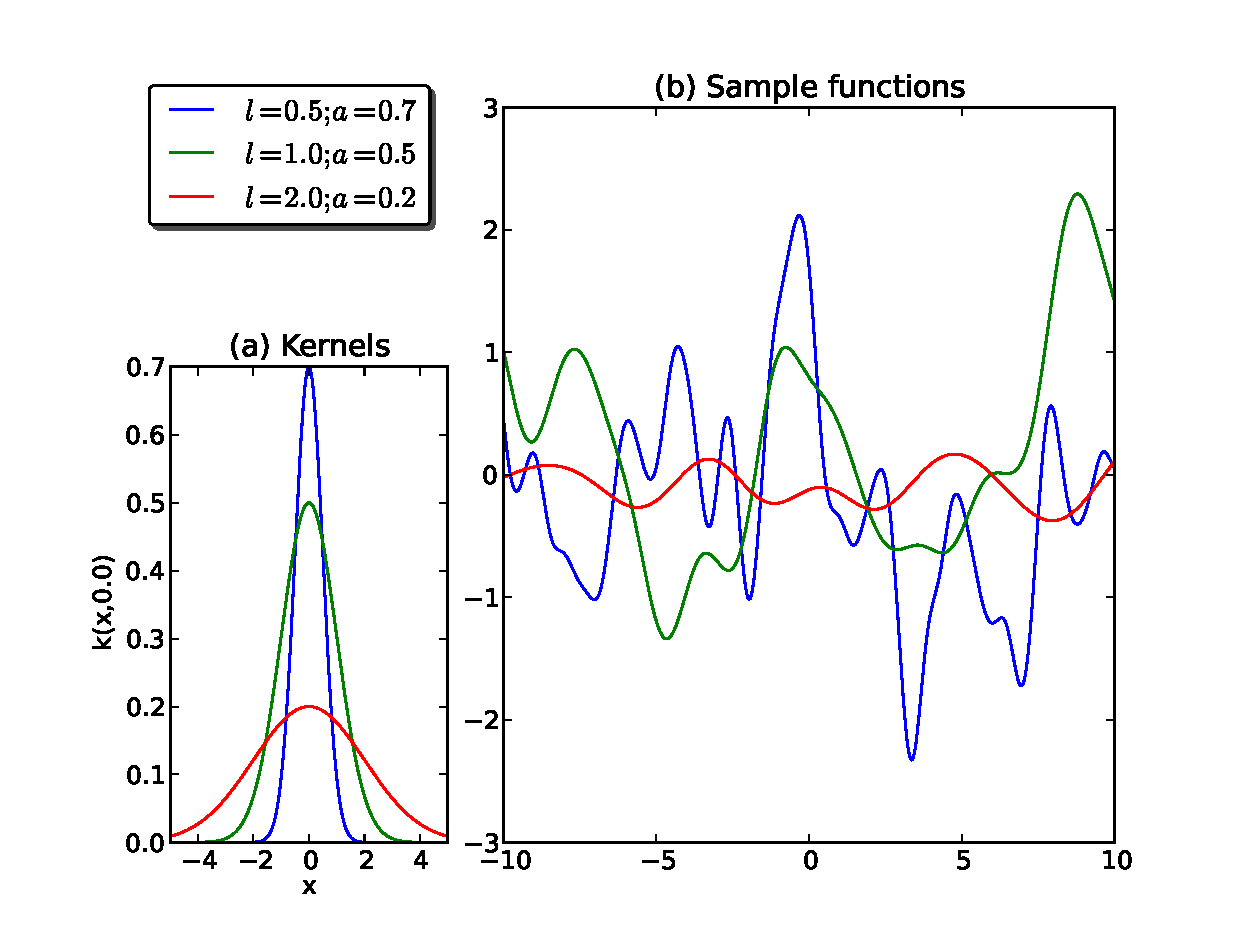
\includegraphics[width=0.9\textwidth,keepaspectratio]{diagrams/SE_cov.eps}
	\caption[Exponentiated Quadratic kernel and sample functions]
		{Exponentiated Quadratic kernel and sample functions}
	\label{fig:Exponentiated_Quadratic_covariance}
\end{figure}

\column{.55\textwidth} % Right column and width
\textbf{The Ornstein-Uhlenbeck covariance function}
\begin{equation} \label{eq:OU}
K_{\nu=1/2}(r)=	\exp \left(-\frac{r}{l} \right)
\end{equation}
\begin{figure}[t]
	\centering
		%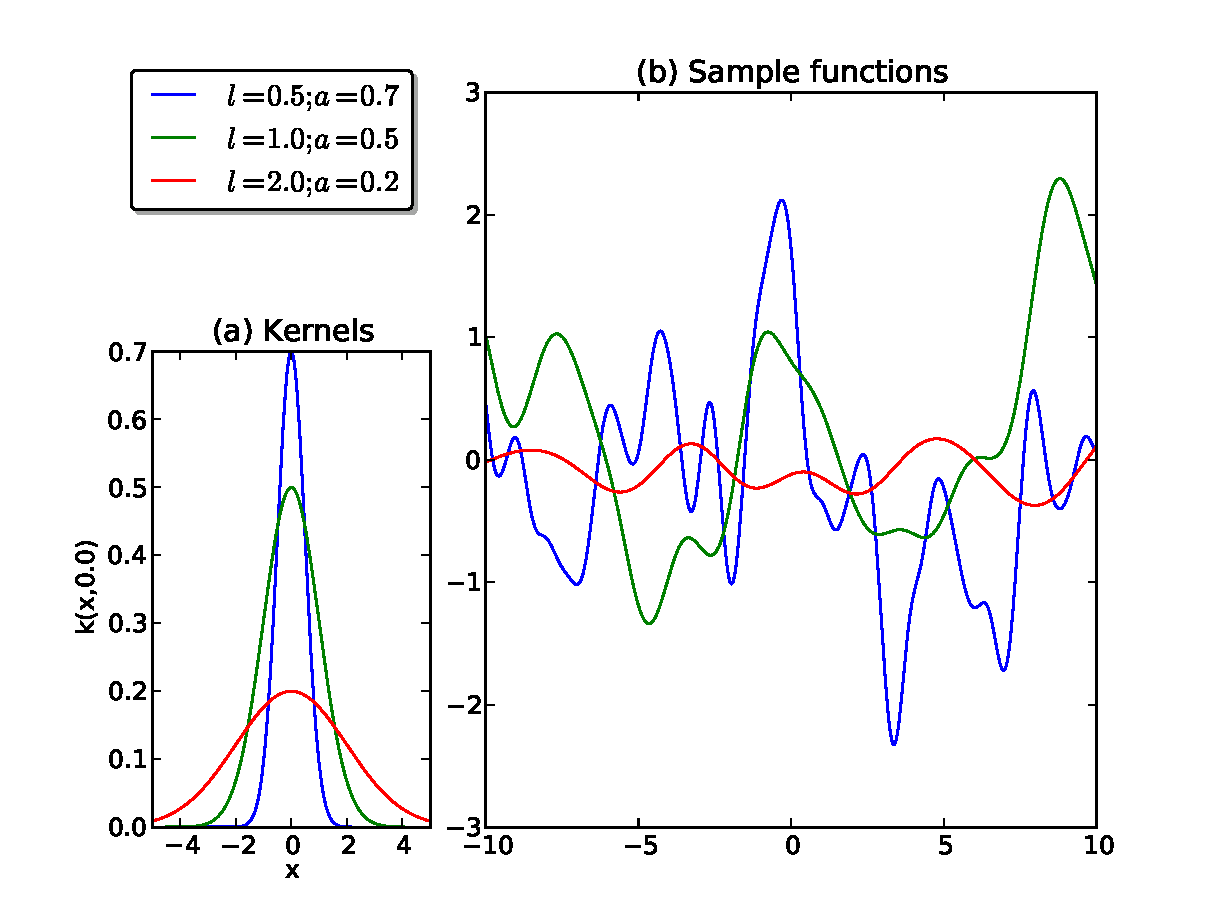
\includegraphics[width=10cm,keepaspectratio]{diagrams/SE_cov.pdf}
		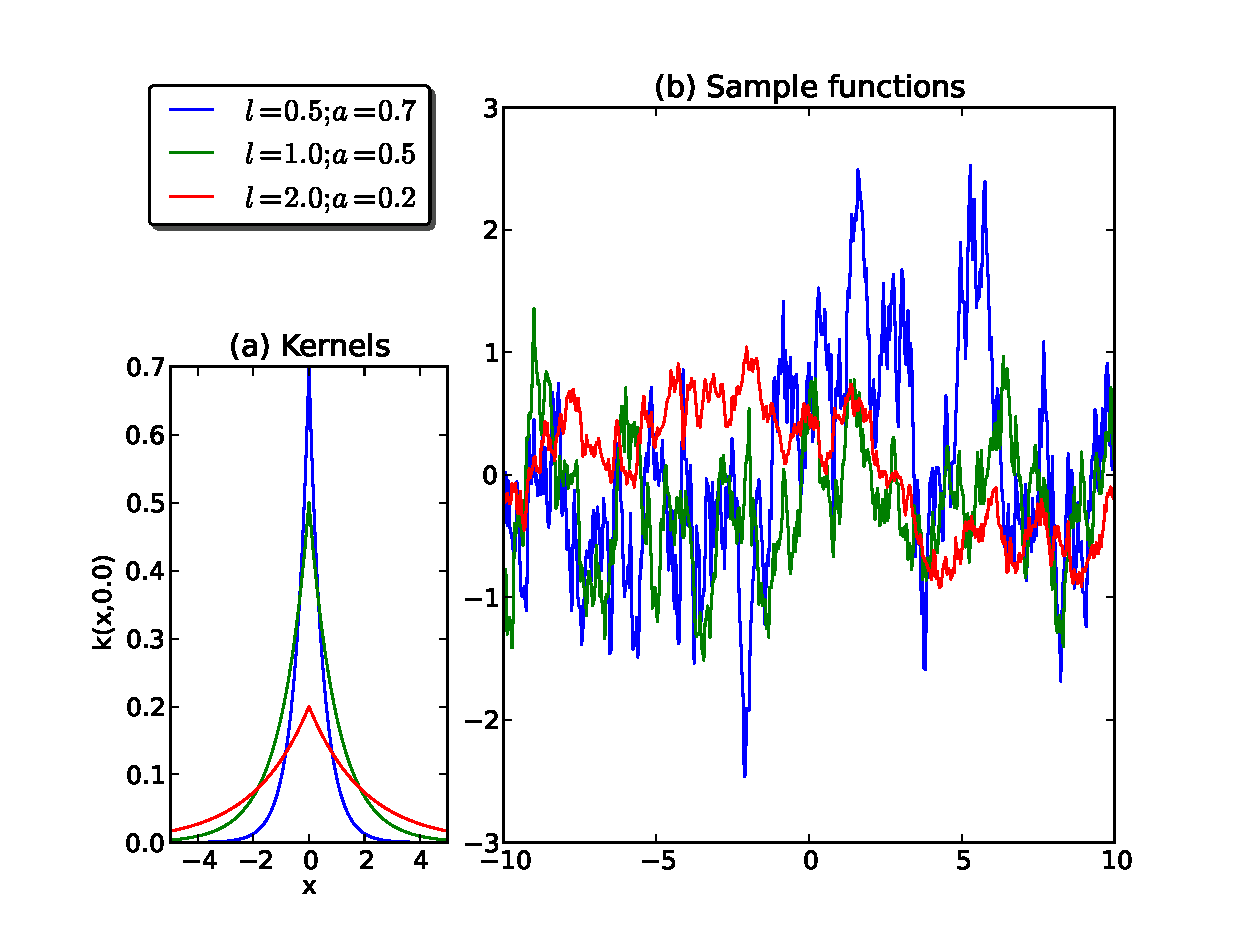
\includegraphics[width=0.9\textwidth,keepaspectratio]{diagrams/OU_cov.eps}
		\caption[The OU kernel and random sample functions]
		{The OU kernel and random sample functions}
	\label{fig:OU_covariance}
\end{figure}
\end{columns}
\end{frame}

%------------------------------------------------
\begin{frame}
\frametitle{Kernels Representation}
\begin{figure}[t]
	\centering
		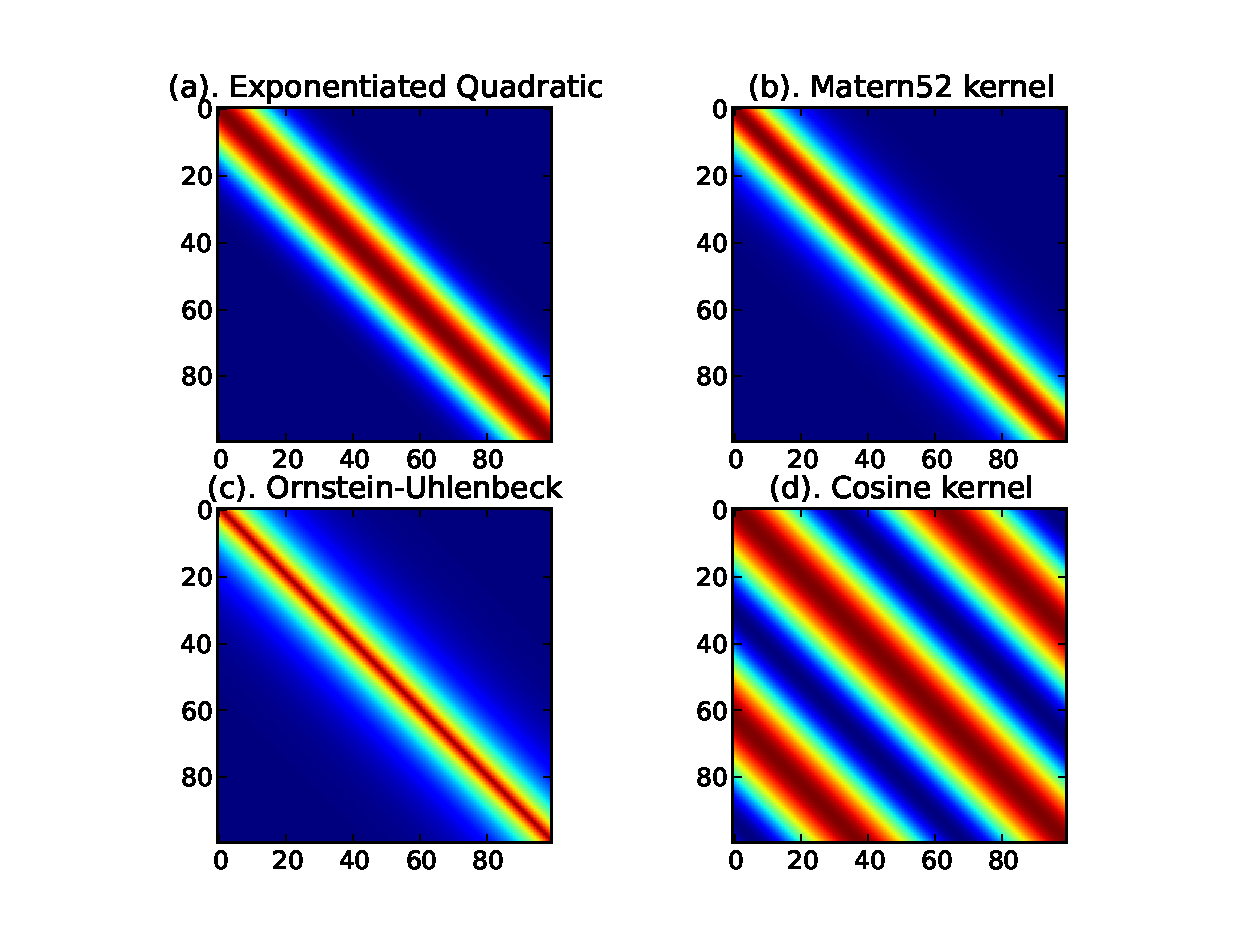
\includegraphics[width=0.7\textwidth,keepaspectratio]{diagrams/DifferentKernels.eps}
		\caption[Representation of some basic kernels ]
		{Representation of some basic kernels (a). Exponentiated Quadratic kernel, 
		(b). Mat{\'e}rn52 kernel (c). Ornstein-Uhlenbeck kernel (d). Cosine kernel  }
	\label{fig:DifferentKernels}
\end{figure}
\end{frame}

\end{document} 